\documentclass{l4proj}
%% Language and font encodings
\usepackage[english]{babel}
\usepackage[utf8x]{inputenc}
\usepackage[T1]{fontenc}

%% Sets page size and margins
\usepackage[a4paper,top=3cm,bottom=2cm,left=3cm,right=3cm,marginparwidth=1.75cm]{geometry}
\usepackage[colorinlistoftodos]{todonotes}
\usepackage[colorlinks=true, allcolors=blue]{hyperref}
\usepackage{listings}
\usepackage{minted}
\usemintedstyle{emacs}
\usepackage{pgfplots}
\pgfplotsset{compat=1.8}
\usepackage{filecontents}
\usepackage{graphicx}
\usepackage{adjustbox}
\usepackage{tikz}
\usepackage{enumerate}
\usepackage{enumitem}
\usepackage{url}
\usepackage{amssymb}
\usepackage{amsmath}
\newcommand{\code}[1]{\texttt{#1}}

\begin{filecontents*}{data.csv}
name map length time
allterms 0.4554  358.5  2.51435
ne 0.3979  93.45  0.4132
tfidf 0.3038  10  0.13675
subject 0.1593  9.75  0.1688
\end{filecontents*}

\title{Public vs. Private: \newline Identifying Public Domain Knowledge}
\author{Kelvin Fowler}
\date{\today}

\begin{document}
\maketitle

\begin{abstract}
The current system of sensitivity review used in the archival process of government documents is slow and insecure. Information Retrieval techniques can be leveraged to vastly improve this operation. This project aims to provide a system and an interface, incorporating these information retrieval techniques, to allow archivists to identify information from documents which already exists within the public domain.
Expand this.
\end{abstract}

% \renewcommand{\abstractname}{Acknowledgements}
% \begin{abstract}
% I would like to thank my supervisors Dr Craig Macdonald and Graham McDonald for their continued assistance throughout the course of this project.
% \end{abstract}

\educationalconsent

\tableofcontents

%%%%%%%%%%%%%%%%%%%%%%%%%%%%%%%%%%%%%%%%%%%%%%
\chapter{Introduction}
\pagenumbering{arabic}

\section{Aims}
This project aims to deliver a prototype of a system which can be used to assist the process of identifying public domain knowledge within potentially sensitive government documents. The project intends to use information retrieval (IR) techniques to present those public domain documents which could help archivists to make an informed choice during sensitivity review. By displaying the information in a document which exists in the public domain an archivist can be sure no new confidential information is being released incorrectly.
The public domain is defined as that information which is available to the public, without legal restrictions, such as news articles.

\section{Motivations}
Document review within government archives faces major problems today. There is a constant barrage of new documents which must be archived and eventually reviewed, driven by the rapid creation of artefacts through technology. Each email and memo is now automatically saved and must, at some point be reviewed.
Further to this, the current system of document review involves no integrated public domain knowledge checking process. Often the substitute for this is a simple web search, which poses many security risks. The search terms themselves could be very sensitive and yet they are being exposed to the internet, and as such, are vulnerable to unintended discovery.
Understanding this, we look to build a system which can keep up with the vast number of documents which need to be reviewed within archives. We also can aim for a system which is encapsulated and secure when it comes to further research on the content of a document.
Combining these concerns we can produce a highly practical and helpful system, which can inspire and encourage further work into this problem domain. To understand further motivations and context behind this project, see Chapter \ref{relatedliterature}.

\section{Terminology}
Throughout this document certain terms will be used which may not be familiar.
A \textbf{Source Document} is the document which is being reviewed. It is the document from which queries are generated for IR.
A \textbf{Target Document} is a document in the public domain which may contain information relevant to the review of a source document. These documents are what we aim to retrieve.

\section{Structure}
This dissertation will take the following structure.
In Chapter \ref{relatedliterature} we investigate the project's relevance through review of some related literature. We then discuss the planning, requirements and design of the system in Chapter \ref{requirementsanddesign}. Chapters \ref{serverimplementation} and \ref{clientimplementation} detail the implementation challenges of the system's components. Chapter \ref{evaluation} explains the experimentation and evaluation undertaken to determine the systems effectiveness. We conclude with learnings and potential future work in Chapter \ref{conclusion}.

\chapter{Related Literature} \label{relatedliterature}
The Freedom of Information Act (2000) allows for all documents held by government to be accessed by the public, upon request, with certain exemptions \cite{foi}. These exemptions are wide ranging, but essentially cover documents which are sensitive for some reason or another. With these exemptions in mind, government must decide if any given document can be released to the public.
The current sensitivity review procedures used by government archivists are less then ideal. Paper documents must be read in full and much interdepartmental conversation must take place before a decision regarding sensitivity can be made. Digital records, of which there are constantly increasing numbers, only make this process even more complicated. This explosion in magnitude poses many potential problems for archiving organisations, such as ``What to Keep?'' and how to effectively identify sensitivities \cite{moss2012have}. The current process is unreasonable and impractical in today's digital context \cite{allan2014record}.

\section{Sensitivity Review}
Some work has already been done to begin to tackle this issue of digital sensitivity review. Prior to review a ``classifier'' may be used to automatically identify potential sensitivities through use of named entities and document sensitivity \cite{mcdonald2014towards}. This type of work can be used to lower the burden on reviewers by attempting to identify documents which may be of the most concern. \\
In other research into the challenges and potential avenues for improving the digital sensitivity review process it was found that document reviewers are reluctant to trust technology alone to identify sensitivities, and that a manual review process will likely always be necessary \cite{gollins2014using}. 
As such, technology which can assist the manual review process (such as that developed in this project) will be increasingly important as the review process is improved and iterated upon.

\subsection{High Recall Tasks}
\todo{How is this stuff relevant?}
High recall tasks focus on retrieving as many relevant results as possible, rather than high precision task which focus on retrieval of results which are most relevant.
One such field where this type of retrieval is particularly sought after is E-Discovery, that is, the discovery of all relevant documents pertaining the opposing party in civil litigation. Information retrieval has been used extensively to provide E-Discovery services \cite{oard2013information}. This application of IR is somewhat analogous to the problem addressed in the project.

\subsection{Entities}
There has been some work into automatically identifying key named entities and concepts within documents. One such work is Wikify \cite{Mihalcea:2007:WLD:1321440.1321475}. Wikify automatically hyperlinks phrases and entities to their relevant Wikipedia articles. A system which can understand and identify the best and most important entities within a document is extremely useful in the context of this project, where we aim to do some kind of searching based on the content of a given source document.

\section{Information Retrieval}
\subsection{Search Engines}
To facilitate the retrieval of public domain target documents from which to draw a conclusion on a source document some form of searching must take place. This is done through a search engine specifically designed for this type of information retrieval. Two such search engines are Terrier and Lucene \cite{macdonald2012puppy} \cite{terrier} \cite{lucene}. These search engines are capable of performing many different tasks outside of the realm of this project, but are configurable to each specific use case. This type of technology is used extensively throughout the project and papers discussed above.

\subsection{Ad-hoc Retrieval}
\todo{Need a source for this section.}
Ad-Hoc Retrieval is IR where there extremely large numbers of potential queries. In our context, we must formulate the best queries possible from our source documents.

\section{The Need for this Project}
In recent times, a great deal more files have been generated by government than ever before. E-mail and digital documents are automatically archived and all must be reviewed and released to the public as mandated by law.  \todo{move this source up in chapter? No sources in this need/gap section?}
Projects such as this one seek to address and help remedy some of these issues by providing efficient and effective tools to ease the digital transition.
The current system of sensitivity review poses potential security risks as sensitive web searches are exposed to the internet. This project provides results in an encapsulated
\begin{center}
\begin{enumerate}[label=\textbf{Need.\arabic*}]
\item Efficient and effective tool to review digital documents.
\item An easier and better way to review public domain knowledge in the context of a source document.
\item Encapsulated environment to do sensitive public domain research.
\end{enumerate}
\end{center}

\chapter{Requirements and Design} \label{requirementsanddesign}
\section{Requirements}
Throughout the project, requirements were identified and categorised using the MoSCoW method. This means that each requirement is identified as either \textbf{Must Have}, \textbf{Should Have}, \textbf{Could Have} or \textbf{Would Like to Have}.
Initially these requirements were elicited from the project supervisors, who have extensive knowledge of the problem domain, through related research and a working relationship with the The National Archives of the UK and Scotland.
These initial requirements allowed the developer to begin work on the project, after which more detailed requirements were identified through discussion and experimentation.

\subsection{Functional Requirements}
The functional requirements of the project were further ratified through user stories. User stories help us to understand why a requirement is necessary and how it benefits the end user. Further to this we can give a more detailed use case to contextualize the following requirements:\\ 
\textit{``Bob is an archivist at the national archives. He must review a collection of emails for sensitivities. Using the new tool he loads up the collection of the emails. When he opens the first email and some relevant news articles are automatically retrieved at the same time. He reads some of the source document and also the top news article. This news article confirms that the content of the email is already in the public domain. Bob classifies the email as not sensitive and opens the next email to repeat the process.''}
\paragraph{Must Have\\}
These are the requirements the the project must fulfil to be considered successful.
\begin{enumerate}[label=\textbf{M.\arabic*}]
\item Allow user to identify when a document contains public domain knowledge. \\
\textit{As a} document reviewer, \\
\textit{I want} the ability to decide that a document contains public domain knowledge \\
\textit{So that} I can make a decision regarding it's status. \\

\item Front end user interface displaying source document for review and target documents automatically identified by the software. \\
\textit{As a} document reviewer, \\
\textit{I want} to view both the document up for review and associated public domain documents \\
\textit{So that} I can easily compare the contents of both and see what is known in the public domain.

\item Trials of different retrieval methods and some form of quantitative analysis based on these. \\
\textit{As a} document reviewer, \\
\textit{I want} to be confident that this software will return the most relevant results in reasonable time, \\
\textit{So that} I can trust the service to return excellent related documents.
\end{enumerate}

\paragraph{Should Have}
These are the requirements which are not vital but are to be fulfilled if possible.
\begin{enumerate}[label=\textbf{S.\arabic*}]
\paragraph{Should Have}
\item Generate suggested queries to allow user to refine returned related documents. \\
\textit{As a} document reviewer, \\
\textit{I want} to refine search terms for related documents, \\
\textit{So that} more relevant documents are returned.

\item Ability to run custom queries. \\
\textit{As a} document reviewer, \\
\textit{I want} to write my own queries, \\
\textit{So that} I can retrieve the best results and be sure that the automatic query system is performing as well as possible.

\item Date range searches. \\
\textit{As a} document reviewer, \\
\textit{I want} to limit date range for retrieval of related documents, \\
\textit{So that} I can ensure relevance of related documents.

\paragraph{Could Have}
These requirements should only be implemented if all of the above requirements have been completed.
\end{enumerate}
\begin{enumerate}[label=\textbf{C.\arabic*}]
\item Machine learning to improve system performance over time based on usage by reviewers. \\
\textit{As a} document reviewer, \\
\textit{I want} my actions using the system to improve it’s performance to better suit my needs, \\
\textit{So that} it is easier to find related documents that I would deem relevant.

\item Tf-idf (Term Frequency - Inverse Document Frequency) analysis to better identify relevant documents. \\
\textit{As a} document reviewer, \\
\textit{I want} to only have returned to me related documents which have been identified as containing search terms in meaningful ways, \\
\textit{So that} I can be sure the returned documents contain information as relevant as possible to the search terms.
\end{enumerate}

\paragraph{Would Like To Have}
These are requirements which are outside the scope of this project and are not deemed important enough to be implemented.
\begin{enumerate}[label=\textbf{W.\arabic*}]
\item Wikify! Like functionality to automatically highlight and link to concepts in source documents which have wikipedia articles associated with them. \\
\textit{As a} document reviewer, \\
\textit{I want} to have easy access to wikipedia articles of items mentioned in the document I am reviewing, \\
\textit{So that} I can easily find out more about concepts mentioned in documents.

\item Eye tracking to automatically identify points of interest in the source document from which to formulate queries. \\
\textit{As a} document reviewer, \\
\textit{I want} the system to react to what my eyes are drawn to, \\
\textit{So that} retrieved target documents are dictated by my actions.
\end{enumerate}

\subsection{Non-Functional Requirements}
Non-Functional requirements are those requirements that do not define the specific behaviour of the system, but rather how the system performs.
\begin{enumerate}[label=\textbf{NF.\arabic*}]
\item Intuitive user interface.
\item Results must be relevant.
\item Must return results in reasonable time.
\item Scalability to handle new large amounts of files. \todo{discuss this somewhere, evaluation?}
\end{enumerate}

\section{Design and Architecture}
The application is based on a client-server design. More specifically, a web application acts as a client which interfaces with a RESTful API acting as a server.
The client communicates with the server using HTTP requests which request information from the server or update information on the server.
The web application maintains no state between usages, but rather requests all necessary data from the server at upon loading. Having no state system in the client application greatly reduces the complexity of the web application.
State and persistence is managed on the server entirely using Terrier and Trec files. This will be discussed in more detail in the Server Architecture section.


\begin{figure}[H]
\centering
\includegraphics[scale=0.50]{images/BigBox}
\caption{Overview of System Architecture}
\label{architecture}
\end{figure}


\subsection{Server Architecture}
\paragraph{Programming Language}
The server component is written in Java. Java was specifically chosen as it was necessary for the server to interact with the Terrier Java API, necessary for the IR features needed to create a viable product.
\paragraph{Information Retrieval}
For the IR needs of the project, Terrier was used. Terrier is a open-source search engine developed at The University of Glasgow, with an extensive Java API allowing it to be easily used for development of various IR tasks \cite{terrier} \cite{macdonald2012puppy}.
Terrier, being developed at The University of Glasgow, was the best and obvious choice of IR technology for the project. The local expertise meant that problems encountered could be easily resolved or explained, ensuring minimal downtime due to learning.
Other potential choices for this section could have been Apache Lucene or MG4J as recommended in Middleton-Baeza's Comparison of Open Source Search Engines \cite{middleton2007comparison}.

\paragraph{Persistence}
One fundamental aspect of Terrier is the concept of indexes. These are files containing the important information from a collection of documents necessary for information retrieval. This provides a persistent data storage mechanism one can use to store additional information about documents or groups of documents. This kind of data is saved in a \textit{meta-index} within a normal index.
The documents pertinent to the project (both source and target) are stored within the server file system as \code{.trec} files. There is one document per file.
These large collections of document files also provide an opportunity to store information. We use this technique to save information too large for the Terrier meta-index.
These techniques produce a fully functional state system capable of retaining all the necessary information needed for the system.
This design entirely eliminates the need for a DBMS (Database Management System) like PostgreSQL and the complicated Java Object to Database Model mapping that often comes with such designs.
We leverage the capabilities of already present technologies to provide persistent state without wasting extensive resources.

\paragraph{Natural Language Processing}
Stanford Natural Language Processing was used as an NLP framework to identify terms from which to form effective queries \cite{manning-EtAl:2014:P14-5}. Provided is a Java API which allows text to be analysed and annotated. More specifically, the named entity identification capability of StandordNLP was used \cite{finkel2005incorporating}.
Stanford NLP was initially chosen due to its preferable documentation. It also offers the ability to identify specifically which tokenisers to use when processing some text allowing the developer to streamline the NLP process to their specific use-case.

\paragraph{RESTful API}
Jersey is a framework which provides a reference implementation of the JAX-RS API as defined by Oracle \cite{jersey} \cite{jaxrsapi}.
Jackson is used alongside Jersey to provide support for JSON \cite{jackson}. This allows the frontend and backend to communicate using one format. It handles the conversion of JSON to Java Objects and vice versa.
This set-up allows one to define a fully functional HTTP REST API which can consume and produce JSON.

\subsection{Client Architecture}
\paragraph{Model View ViewModel}
The architecture of the front end user interface is based around the Model View ViewModel (MVVM) design pattern. Facilitated by the JavaScript library Knockout.js, MVVM allows us to consolidate the logic associated with the DOM (Domain Object Model) into one place \cite{knockout}.
We no longer need to apply JQuery or Vanilla Javascript to individual DOM elements through classes and ids, but instead we can apply rules identified in the ViewModel to various elements throughout the DOM. This allows for dependency tracking of JS variables and automatic real time updates as their values change.
This lends itself well to the problem domain of many rapidly changing documents and results sets as the user identifies relevant documents. \\
Knockout was chosen due to developer familiarity. There are various other libraries that allow for similar designs, however familiarity with Knockout's syntax and best practices meant that development was easy and fast.
This was important as the learning curve for the backend technologies required more attention, and so ease of development on the frontend was key.

\paragraph{Style}
Although our data manipulation is handled by Knockout we present this information in an intuitive and user friendly way. There are many frameworks which provide pre-built components to build user interfaces but Bootstrap was chosen mainly due to familiarity reasons. It provides myriad customisable components, as well as being extremely well documented \cite{bootstrap}. This dramatically simplifies the rapid development of a user interface.

\paragraph{AJAX}
JQuery is used in the frontend to interface with the backend through HTTP (AJAX) requests. JQuery provides a very well documented and widely adopted API for this. JQuery is a dependency of both Knockout and Bootstrap and so utilizing it's already present features was sensible and easy.

\paragraph{Web Application Framework}
The web application currently runs on top of an Express.js server running on Node.js \cite{express} \cite{node}. This is not particularly necessary as the web application could, with some refactoring, be served through a static web server such as GitHub Pages. What Express.js does allow for, however, is the use of the EJS template system. EJS allows us to define partial HTML pages and insert them into others. This is useful within the MVVM design as we can initialize compartmentalized parts of the DOM with specific ViewModels using the \code{with} binding, see section (\ref{viewmodels}) for more details.

\todo{Wireframing and Prototyping ++ Images}

\section{Conclusion}
With these we requirements and design decisions in mind we look, in the next two chapters, at how they they were implemented and the challenges that arose during this. In Chapter \ref{evaluation} we also investigate if the requirements were fulfilled and how effective the implementation of the system was.

%%%%%%%%%%%%%%%%%%%%%%%%%%%%%%%%%%%%%%%%%%%%%%%
\chapter{Server Implementation} \label{serverimplementation}
This Chapter will discuss the implementation of the server component of the system. It will cover in detail the use of Terrier to index and retrieve target documents as well as how queries were generated. Also covered is the implementation of the RESTful API to allow communication with the client.

\begin{figure}[H]
\centering
\includegraphics[scale=0.50]{images/ER-IPDK}
\caption{Entity Relationship Diagram for Documents}
\label{er}
\end{figure}

\section{Tools}
\paragraph{Git and GitHub}
Git was used, alongside GitHub as Source Control Management (SCM) for the project \cite{git} \cite{github}. This allows one to maintain version history for the project. Hosting the repository on GitHub also served as a back-up for the project, and allows it to be cloned onto any machine.
\paragraph{Trello}
Trello was used throughout the project to plan implementation steps and track bugs. \cite{trello}.
\section{Dependency Management and Build System}
Maven was used as a dependency management and build system \cite{maven}. Maven was chosen due to it's ease of use and clear documentation. It allowed for easy inclusion of all the dependencies needed for the project such as Terrier, StanfordNLP and Jersey. Maven's build system also ensures all unit and integration tests pass before building the system into a runnable jar file.

\section{Data}
\subsection{Source Documents}
\todo{discuss this in experimental set-up section of evaluation, also don't have to directly mention wikileaks.}
During development the collection of source documents used for testing and experimentation was based upon the United States Diplomatic Cables Leak, as released on Wikileaks. This collection has been confirmed to be relevant and very similar to the type of documents reviewed by the archives services in the UK \textbf{do you have a source for this?}. The documents were provided in TREC format, with one document per file. They were arranged into directories based on year and month of creation.
\begin{minted}{xml}
<DOC>
<DOCNO>08ABUDHABI1104</DOCNO>
<CREATED>2008-09-28</CREATED>
<RELEASED>2011-08-26</RELEASED>
<CLASSIFICATION>UNCLASSIFIED//FOR OFFICIAL USE ONLY</CLASSIFICATION>
<ORIGIN>Embassy Abu Dhabi</ORIGIN>
<FROM>AMEMBASSY ABU DHABI</FROM>
<TO>RUEHC/SECSTATE WASHDC 1507</TO>
<SUBJECT>UAE PRESIDENT DEPLOYS PERSONAL CHARITY FOUNDATION </SUBJECT>
UAE PRESIDENT DEPLOYS ...
</DOC>
\end{minted}
\subsection{Target Documents}
A combination of Associated Press and Reuters articles were used as target documents to perform retrieval on. These were again in TREC format, with one file per document. They were also each compressed due to the extremely large number of them.
They were given in the following format:
\begin{minted}{xml}
<DOC>
<DOCNO>trc2_168664420090204</DOCNO>
<TITLE>GLOBAL MARKETS-Economy hopes boost stocks, dollar</TITLE>
<DATE>2009-02-04</DATE>
<KEYWORDS> MARKETS GLOBAL   </KEYWORDS>
* Global stocks rise on economy hopes...
</DOC>
\end{minted}
\section{Indexing}
Through the Terrier API, collections of documents can be indexed. Indexing identifies the correct terms within documents to match search queries on, as well as performing other processes necessary for IR. Indexing uses a tokeniser to produce tokens from words and feed them to these processes and add them to the index.
\subsection{Named Entity Tokeniser} \label{nertok}
We wanted to identify Named Entities within documents to enhance query generation and provide better retrieval. \\ 
This provided a hook-in point for named entity identification as we can identify if terms are Named Entities before they are passed out of the tokeniser to be added into the index.
A custom subclass of the Tokeniser class in Terrier was implemented which applied named entity identification to a document body before being tokenised.
If a term was identified to be a named entity by Stanford NLP then an underscore and the named entity type was appended to the terms. For example, 
\code{kelvin} becomes \code{kelvin\textunderscore person}. \\
The logic for annotating a section of text was further abstracted to a separate class so that it could be reused to annotate any text, outside of the context of tokenisation during indexing. This was used specifically to annotate subject queries in the query generation phase, but could provide further applications in the future.
\paragraph{Classifiers and Distributional Similarity} \label{classifiers}
An instance of \code{StanfordCoreNLP} must be created to use the named entity annotation features.
In this instance the fewest possible annotators were used to acheive named entity recognition.
We use the simplest classifier model provide by StanfordNLP which only looks for Location, Organisation and Person named entities.
As discussed in the evaluation section, we also tried Named Entity models with and without Distributional Similarity Features (The documentation suggests this can improve performance while sacrificing efficiency).
We also avoid time and numeric entity identification, so as to only focus on the tangible entities mentioned throughout each document.

\subsection{Target Documents}
The system operates on the assumption that there already exists a target index within it's directory structure.
As such, a separate Java program was written which can index target documents through command line invocation. The program loads the appropriate Terrier properties and invokes indexing through Terrier's API. \\ During target document indexing we set the Terrier properties so as to create abstracts. Abstracts are parts of a tagged document to be saved in meta-data to provide helpful snippets of the document when it is found during retrieval. In this case, we generate abstracts for the title, data, keywords and body of the document to give an idea of document contents when looking at query results.
The correct configuration of Terrier to achieve this caused considerate trouble during development and was actually the identifier of a flaw in Terrier itself. Owing to the fact that the project supervisor was a key Terrier developer, this was fixed through a patch and the target index could be generated correctly.
As target document indexing uses the same tokeniser (see section \ref{nertok}) as source document indexing, we can guarantee term matching across the two corpora when performing retrieval.

\subsection{Source Documents}
In order to find the terms necessary to formulate queries we must also index the source documents.
Source indexing is invoked through the REST API. Again this loads the relevant Terrier properties and invokes indexing through the Terrier API. The Terrier properties important to this operation are the \code{TrecDocTags.PropertyTags}, which identify the tags in a tagged document which are to be saved as document properties, rather than being indexed. We only index the main body of each document. Additionally, source indexing also invokes query generation (see section \ref{querygen}). 

\subsection{Query Generation} \label{querygen}
Immediately after indexing a collection of source documents, the system invokes the query generation process. We create 4 queries: All Terms, Named Entity Terms, Top Ten Tf-Idf Named Entities and Subject Queries.
Throughout this section we will use this document to give examples of the generated queries:
\begin{minted}[breaklines,breaksymbolleft={}]{xml}
<DOC>
<DOCNO>08LONDON2702</DOCNO>
<CREATED>2008-10-27</CREATED>
<RELEASED>2011-02-04</RELEASED>
<CLASSIFICATION>CONFIDENTIAL</CLASSIFICATION>
<ORIGIN>Embassy London</ORIGIN>
<FROM>AMEMBASSY LONDON</FROM>
<TO>RUEHC/SECSTATE WASHDC 0217</TO>
<SUBJECT>UK WILL NOT PARTICIPATE IN IRAN'S NUCLEAR CONFERENCE, WILL DISCOURAGE OTHERS FROM ATTENDING REF: STATE 112229 </SUBJECT>
UK WILL NOT PARTICIPATE IN IRAN'S NUCLEAR CONFERENCE, WILL DISCOURAGE OTHERS FROM ATTENDING REF: STATE 112229

Classified By: Political Counselor Rick Mills for reasons 1.4 b and d (C)

 HMG does not intend to participate in Iran's November 30 nuclear conference, since attendance would "give credibility" to Iran's claims about its nuclear activities, Foreign and Commonwealth Office (FCO) Counterproliferation Department officer Lesley Craig told Poloff October 24. Craig said the FCO will tell anyone who contacts HMG about the conference, such as academics and NGOs, that it would be advisable not to attend. She added that the UK probably would not do a "formal demarche" to other countries regarding non-attendance; she suggested that countries likely to attend the conference would not be amenable to a demarche in any event. Separately, FCO Iran Coordination Group Regional Team Leader Rachel Martinek made comments to Poloff consistent in substance with all Craig's points. Visit London's Classified Website: XXXXXXXXXXXX TUTTLE
</DOC>
\end{minted}
\paragraph{Subject Query}
\begin{minted}[breaklines,breaksymbolleft={}]{xml}
uk will not participate in irans_location nuclear conference will discourage others from attending ref state 112229
\end{minted}


\paragraph{Tf-Idf Named Entities Query}
\begin{minted}[breaklines,breaksymbolleft={}]{xml}
craig_person fco_organization hmg_organization participate_organization martinek_person lesley_person counterproliferation_organization iran_location rachel_person rick_person
\end{minted}

\todo{Where do you first mention the 4 queries that we want to create (initially anyway)?}
\paragraph{All Terms Query and Named Entities Query}
To create the All Terms and Named Entity Queries we simply iterate through the terms in the index for a given document and append them to a \code{StringBuilder}. One \code{StringBuilder} amalgamates every term found, while the other only takes terms containing an underscore, the identifier for a named entity found during indexing using the \code{NamedEntityTokeniser}. 
\paragraph{Named Entities Query}
\begin{minted}[breaklines,breaksymbolleft={}]{xml}
state_location iran_location foreign_organization department_organization group_organization uk_location political_organization office_organization regional_organization coordination_organization poloff_person c_organization london_location conference_organization mills_person ngos_organization team_organization october_person nuclear_organization november_organization will_person iran_organization visit_location hmg_organization counselor_organization will_location commonwealth_organization xxxxxxxxxxxx_person conference_location nuclear_location rick_person craig_person rachel_person fco_organization participate_organization martinek_person lesley_person counterproliferation_organization
\end{minted}
\paragraph{All Terms Query}
\begin{minted}[breaklines,breaksymbolleft={}]{xml}
s countries lrb  state_location who  rrb   will 24 participate made tell event 30 told attending  give suggested demarche iran_location added officer ref foreign_organization department_organization likely formal  nuclear group_organization reasons conference comments attend uk_location political_organization office_organization regional_organization discourage coordination_organization activities poloff_person claims classified 14 c_organization london_location points separately conference_organization mills_person leader consistent ngos_organization team_organization october_person contacts nuclear_organization website november_organization advisable intend substance will_person attendance iran_organization credibility visit_location hmg_organization counselor_organization academics will_location commonwealth_organization xxxxxxxxxxxx_person conference_location nuclear_location 112229 rick_person craig_person amenable rachel_person nonattendance fco_organization tuttle participate_organization martinek_person lesley_person counterproliferation_organization
\end{minted}

For the Tf-Idf query we leverage the Terrier API which has methods to give us all the data we need.
Tf-Idf (Term Frequency - Inverse Document Frequency) is defined as:
\begin{gather*}
Tf\textnormal{-}Idf = Tf \cdot Idf \\
\textnormal{where:} \\ 
Tf = \frac{Number\ of\ Times\ Terms\ Appears\ in\ Document}{Total\ Number\ of\ Terms\ in\ Document} \\ \\
Idf = \ln{\frac{Total\ Number\ of\ Documents\ in\ Collection}{Number\ of\ Documents\ Containing\ Relevant\ Term}}
\end{gather*}
For any given term we can retrieve it's term and document frequency in order to easily calculate the Tf-Idf of the term. Once calculated the term and value are inserted into a data structure from which retrieve the top-ten terms to formulate the query.\\
The subject of the document is not indexed and not stored in the meta-index. This is due to it's unpredictable length (Terrier can only save fixed lenght meta-index items). We create the subject query at source document load time. When the API gets a request to return the source document we invoke named entity analysis on the subject found in the document. It is then stripped of punctuation, converted to lower case and saved in an instance field to be passed as JSON to the client. Due to needing a StanfordNLP instance to create the subject query the first source document loaded can often take slightly longer than the others. This is an unavoidable inconvenience at the moment, due to the static StanfordNLP instance needing to instantiated at somepoint in time.\\

Having formulated all four queries we wrap them in tags and append them to the end of the trec source document from which they were generated. This allows the process described in section \ref{docparse} to find the queries without the need for any new storage mechanisms.

\paragraph{Available Indexes}
Since we can index individual directories of source documents, a tool to choose which collection to review must also be provided. This functionality relies on a system of recursive file finding. We simply look in index directories until we find a \code{collection.spec} file indicating an index is present. This relative path can be used to give the directory of source documents in the \code{collections} directory as the this and the index directory are exact mirrors of each other.

\section{Retrieval}
Retrieval is a fairly simple affair, almost identical to the provided example retrieval code provided in the Terrier documentation.
\paragraph{Decoration}
At this stage we also leverage Decoration, a functionality provided by Terrier to highlight and emphasise terms within a result set which appear in the query. Conveniently the decoration wraps found terms in \code{<b>} HTML tags, allowing us to render them as bold in the frontend.

\section{Document Parsing} \label{docparse}
In order to display the source and target documents to users on the front end they must be parsed and converted to JSON.
Both target and source documents are provided in TREC format with various meta-data tags and an untagged body section.
An abstract class, \code{TaggedDocument} was created which reads these documents identifying tag types and content. Once identified, this method can pass the tag type and tag content to the concrete subclass which implements a method to match tag types and put the content in an instance variable ready to be serialized to JSON and sent to the client.

\section{Evaluation Preparation}
In order to prepare the \code{.topics} and \code{.qrels} files necessary for offline evaluation.

\section{API Design}
The API is designed as follows:
Get Source Document
\code{GET api/document/{sourceCollectionPath}/{docId}}
Get Target Document
\code{GET api/document/{docNo}}
Index a Source Collection
\code{POST api/index}
Query the Target Index
\code{POST api/query}
Get Indexed Source Corpora
\code{GET api/index}
Save a document and queries to topics
\code{POST api/topic}
Save a judegement on a target document for a given source document
\code{POST api/qrel}
Get those target documents which are already judeged for a given source document
\code{GET api/qrel/{num}}

\section{Properties}
Terrier operates with a collection of properties which change the behaviour of it's various operations. These properties can be set inside a terrier.properties file, however this complicates changing these properties between different operations. These properties can be set programatically and so a static class was made which allows for easy switching of settings to facilitate correct invokation of indexing and retrieval. : Talk about Source vs. Target indexing

\section{Summary}
Was query generation effective?
Is the system scalable?
Did NLP models effect the query results?
Is the system fast?

%%%%%%%%%%%%%%%%%%%%%%%%%%%%%%%
\chapter{Client Implementation} \label{clientimplementation}
This chapter will deal with the steps taken in the implementation of the web application which acts as the client in the client server paradigm.

\section{Tools and Methods}
\paragraph{Dependency Management}
Bower was used for dependency management within the realm of frontend JavaScript. Bower allows a programmer to define dependencies through a \code{bower.json} file. These can then be downloaded through a bower install command straight into a bower components folder. This was used to install JQuery, Bootstrap and Knockout.

\paragraph{IDE}
JetBrains WebStorm was used to develop the client web application. It allows for easier and faster development by allowing one to run a Node.js application through it's interface, as well as other niceties such as intelligent code completion.

\section{ViewModel and Data Binding} \label{viewmodels}

\section{Computed Functions and Observables}
Within the ViewModel, the programmer defines Observables instead of plain JS variables. These ensure inclusion of the logic needed to interact with the DOM through data-binding. Observables can also be ``computed". This means that their value depends on an automatically evaluating function. These functions re-evaluate any time an observable which is a dependency to the function changes. This system allows for complex logic which can be fired off automatically depending on certain circumstances.
This feature can also be exploited to allow for automatic firing of events not related to any specific observable. This is very useful in this project's context as we can send off API requests when certain observables change, for example the requested source document.

\section{Components for Tab System}
Knockout provides a component system which allows one to register new html elements, along with a specific view model with which these objects interact. The programmer provides a html template (complete with data-binding) and a ViewModel. When instantiating one of these components one passes in arguments to fill the ViewModel.
This system lends itself excellently to the tab system present in the system. Using a ``foreach" binding along with these custom components a fully functional tab system exists, which is, at it's foundation, simply an array of docNo's. Such is the power of declarative bindings and custom components! Haha!

\section{Decoration}
We use css to highlight in red those terms which we appear in the query and are in the target documents. 
\begin{minted}{css}
.decorate > b{
    color: red;
}
\end{minted}

\begin{figure}[H]
\centering
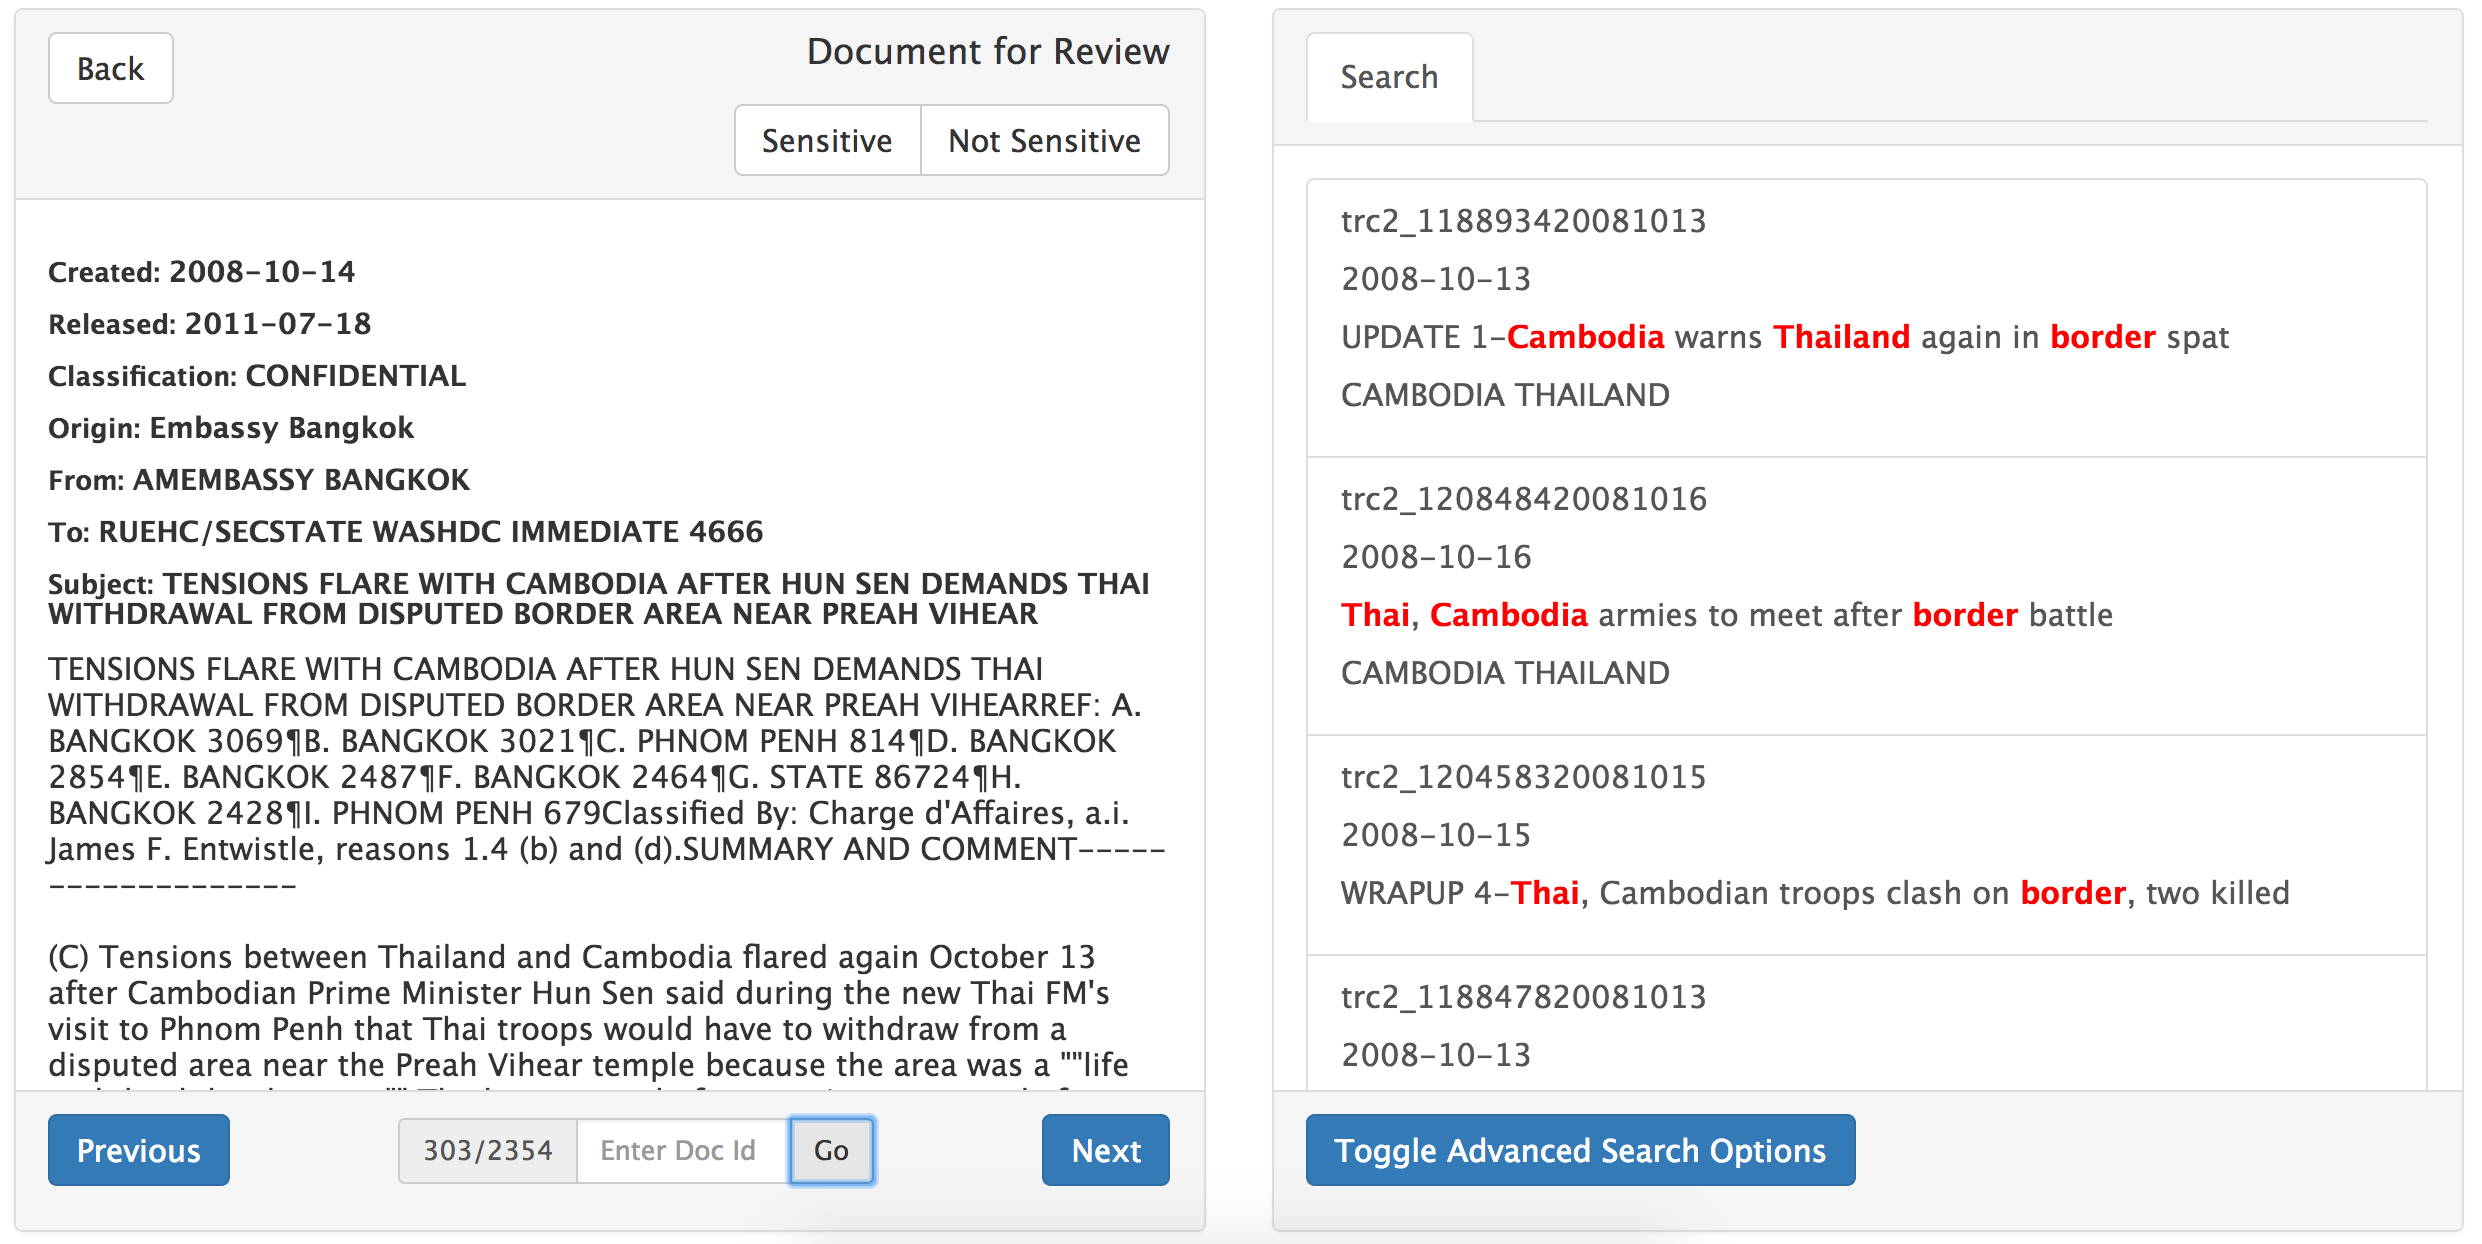
\includegraphics[scale=0.30]{images/searchresults}
\caption{The Front-End Search Results}
\label{relevant_results}
\end{figure}
\begin{figure}[H]
\centering
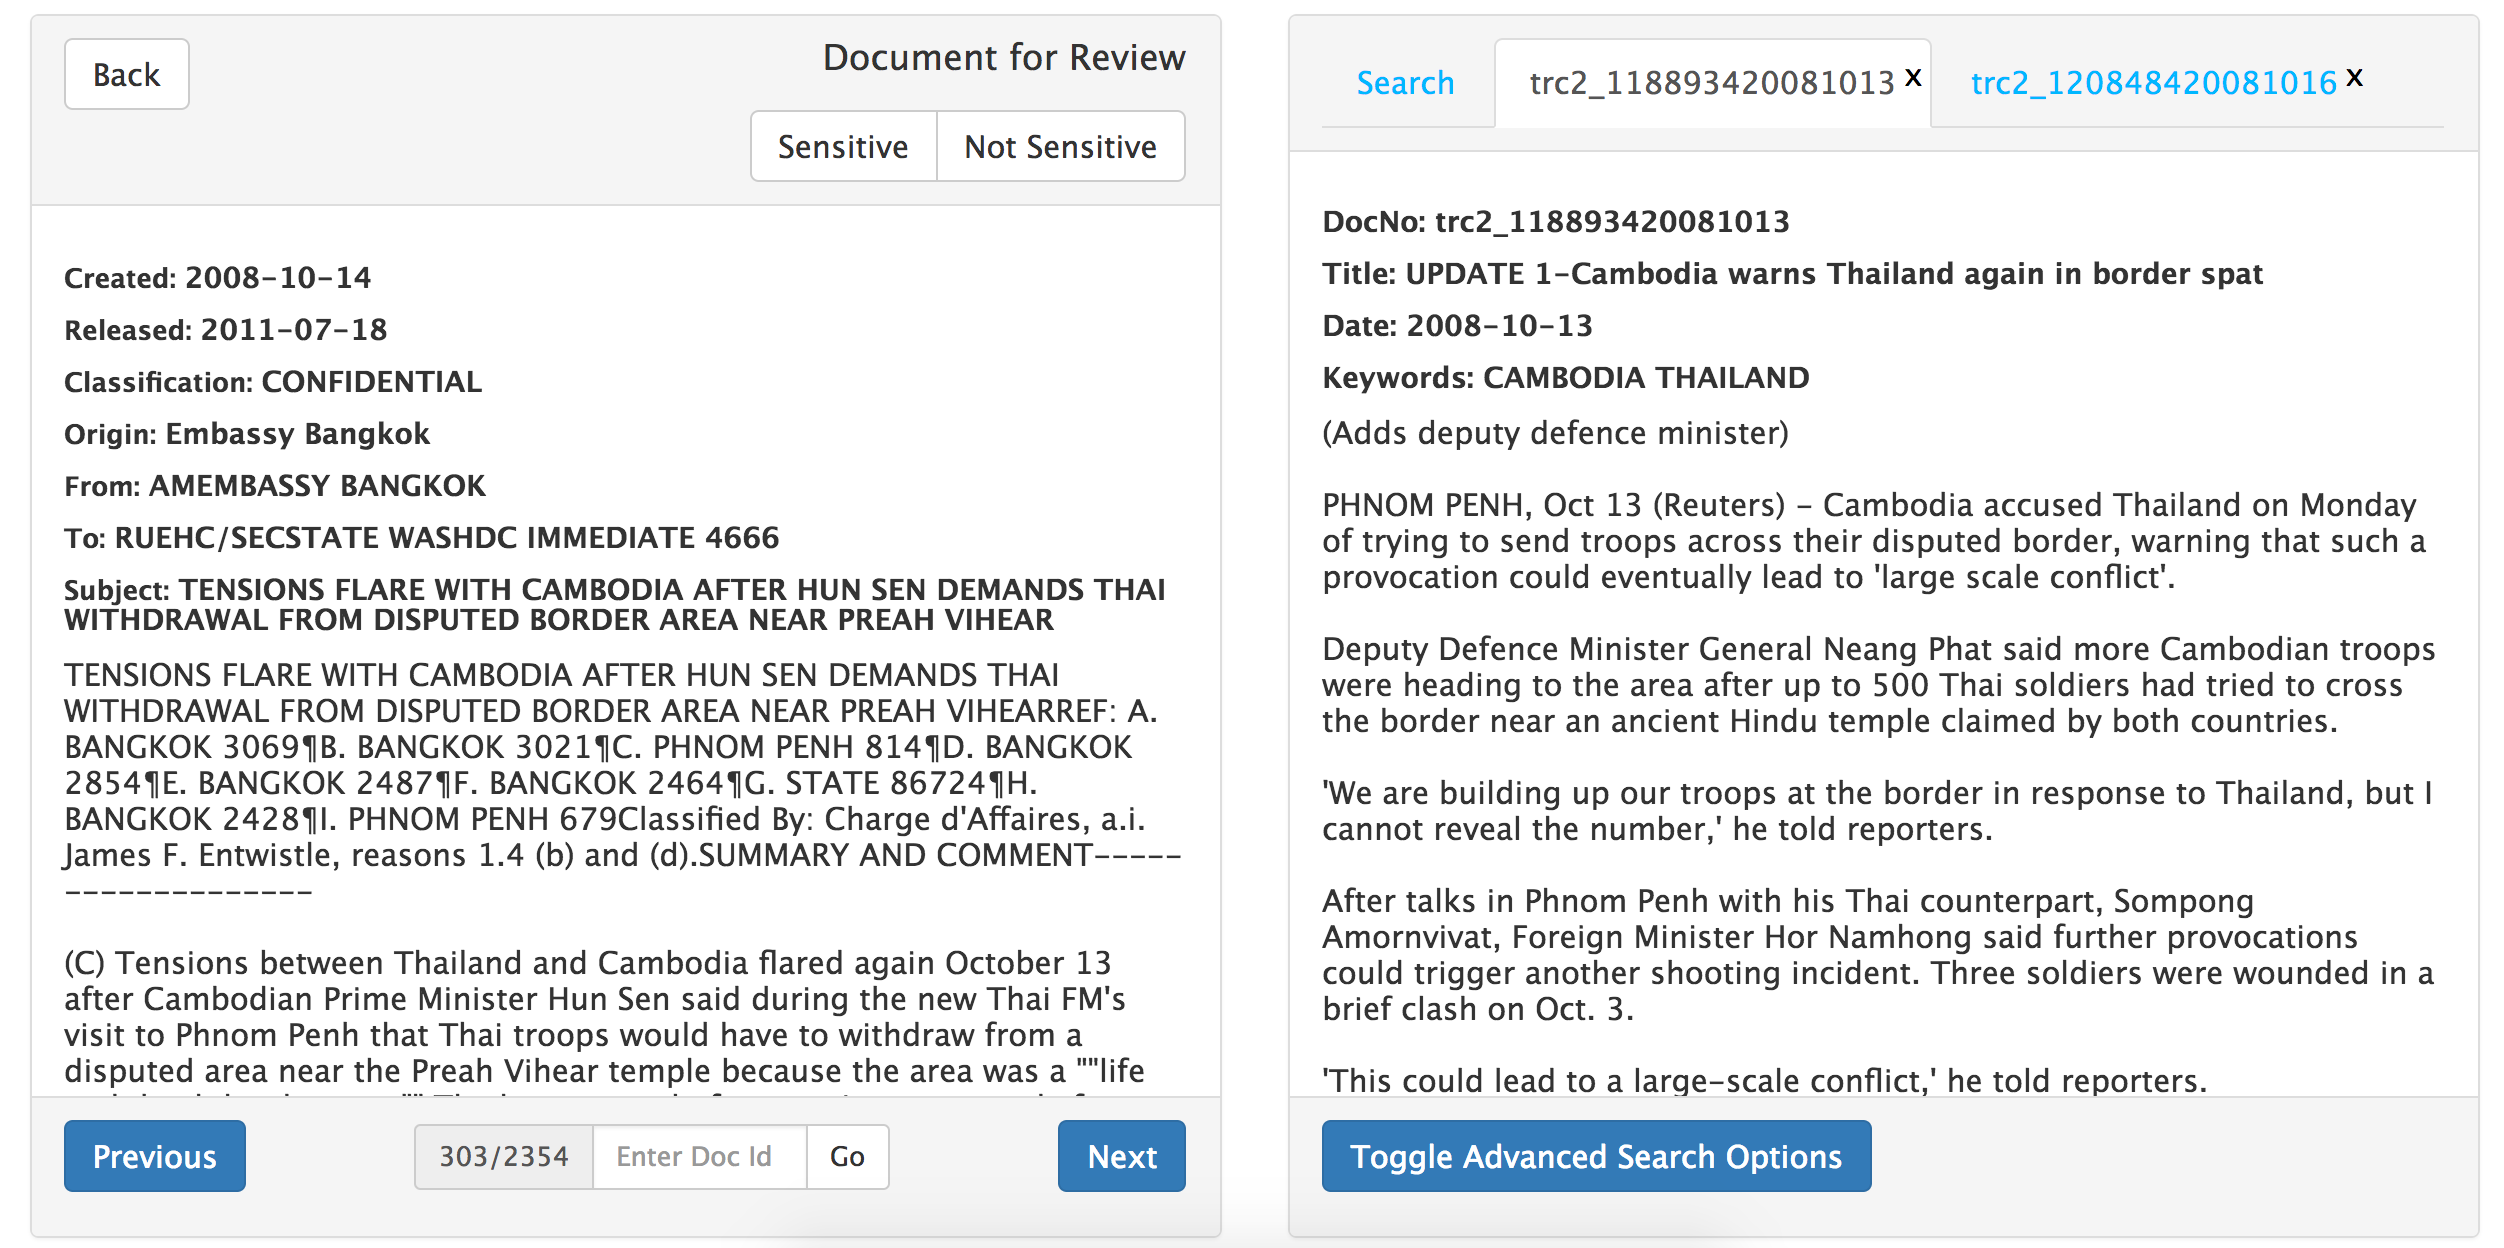
\includegraphics[scale=0.30]{images/targetdocument}
\caption{Viewing a Target Document}
\label{relevant_results}
\end{figure}

\section{Summary}
In order to validate user acceptance testing it was decided that variants of the front end system were to be created. These variants would play on some of the main features of the frontend design, in order to identify the UI elements which were helping and hindering the user experience.

%%%%%%%%%%%%%%%%%%%%%%%%%%%%%%%%%%%%%%%%%%
\chapter{Evaluation} \label{evaluation}
\todo{fix requirement references}
In this chapter we will discuss the various stages of evaluation and experimentation performed on the system.
We investigate Unit Testing in section \ref{testing} to ensure the system is robust (fulfilling NF5).
In section \ref{offlineevaluation} we experiment with the best query to fulfil Must Have Req Automatic queries \todo{fix} and the other requirement.
And finally in section \ref{userevaluation} we look into the thoughts of a potential user of the system and how the UI can be improved for usability to better satisfy \textbf{NF1}.
\section{Testing} \label{testing}
\subsection{Unit Testing}
JUnit was used to organise and run unit tests on the various classes present in the backend application.
The Arrange-Act-Assert pattern was used to organise unit tests in a structured way. This arrangement allows for clear identification of the method being tested, separate from the code needed to prepare for the test.
Testing necessitated the refactoring of some of the files which read and write information to files. Let us observe an example in the form of the TargetDocument.java class. This class analyses a compressed target document to create a representation which can be converted to JSON and delivered to the Web App for viewing.
The constructor originally took a file path and constructed the necessary streams and readers to allow for reading of the file.
\begin{minted}{java}
public TargetDocument(String path){
  try {
    FileInputStream stream = new FileInputStream(path);
    GZIPInputStream gzStream = new  GZIPInputStream(stream);
    InputStreamReader inputStreamReader = new  InputStreamReader(gzStream);
    BufferedReader br = new  BufferedReader(inputStreamReader);
    documentParser(br);
...
\end{minted}

This approach is inflexible as it assumes the file path will direct to a gzipped file. It means that unit tests need either a sandbox file system to prepare tests, or some kind of mocking of the file system. Mocking a file system is overly complex and adding a sandbox filesystem adds unpredictable side effects.
A better, more general, and self contained approach is to have the constructor take a \code{Reader} interface as an argument. We can then instantiate the necessary \code{BufferedReader} needed.

\begin{minted}{java}
public TargetDocument(Reader r){
    BufferedReader br = new BufferedReader(r);
    this.docNo = this.title = this.date = this.keywords = this.body = "";
    documentParser(br);
...
\end{minted}

This approach was extended to several classes which handle interacting with files.
Code which interacted with the Terrier API posed problems in term of unit testing. Terrier often introduces side effects in the form of interacting with established index files in the file system.
\section{Qualitative Analysis and Defining Relevance}
Through the course of developing the system and producing the ground truth necessary for the Offline Evaluation as discussed in the next section, certain nuances of the system became clear. \\
It was clear that named entity analysis was certainly not always full proof. Sometimes entities were missed and often words such as ``and'' or ``the'' were tagged as named entities incorrectly. Combating this, the variations of ``and'' and ``the'' created in the named entity identification process were added to the stopwords file to avoid them appearing in queries and being matched in retrieval. \\
In order to produce the \code{qrels} file it was necessary to define returned target documents as ``relevant'' or ``not relevant''. This was extremely nuanced and relied on the discretion of the reviewer. Look at the following example of target documents returned for a source document regarding border clashes between Thailand and Cambodia:
\begin{figure}[H]
\centering
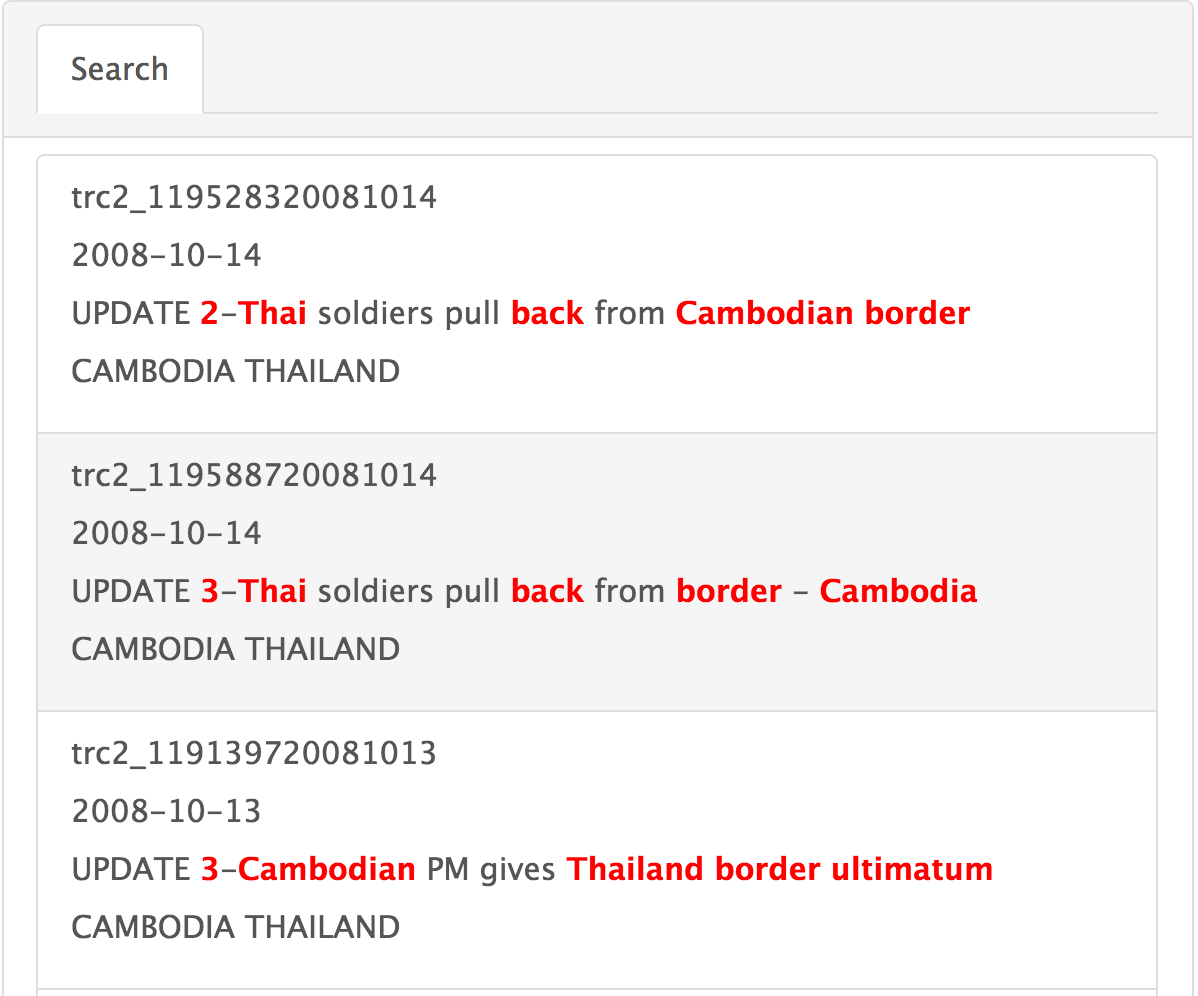
\includegraphics[scale=0.30]{images/good_results}
\caption{Recognisable Relevant Results}
\label{relevant_results}
\end{figure}
\begin{figure}[H]
\centering
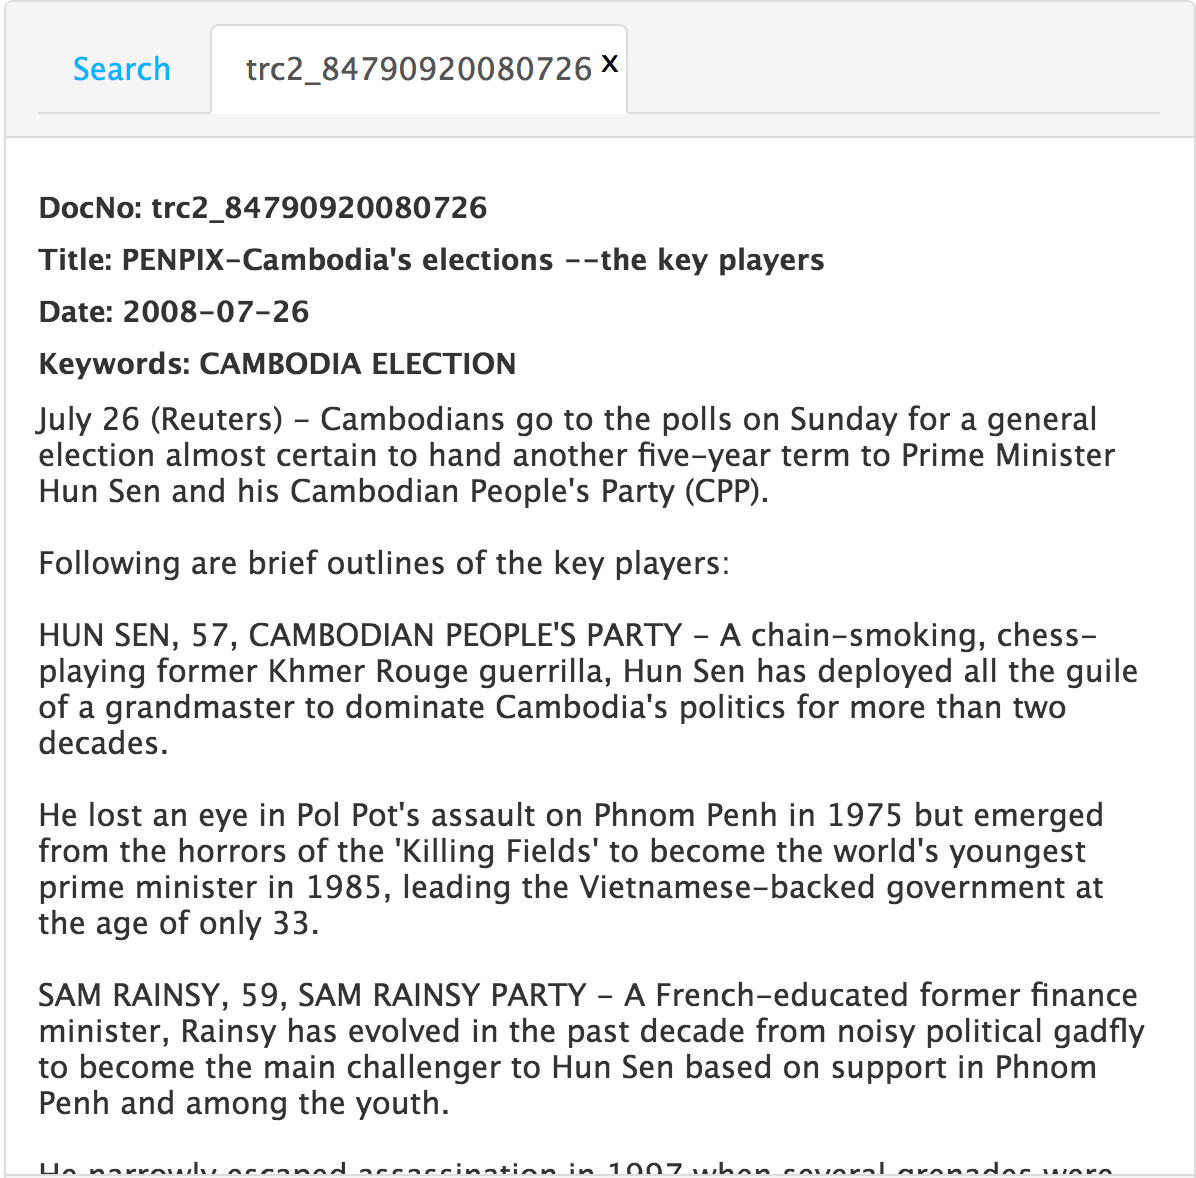
\includegraphics[scale=0.30]{images/bad_result}
\caption{An Irrelevant Result}
\label{irrelevant_result}
\end{figure}
\bigskip

It is clear why the result shown in \ref{irrelevant_result} was returned from some formulation of a query, as it mentions Cambodia and the Prime Minister Hun Sen. Sometimes, this was not as clear cut and things like date's were important. An example is an article regarding ``Fighting in North Darfur''. The event being referred to was around a specific date, and so we had to ensure any target document pertaining to fighting in North Darfur matched the correct time frame. \\
The query formed from Tf-Idf ranking of named entities was interesting. It often produced relevant results, but was also the cause of many strange results, such as reports on international sports fixtures. One can see how this occurred, since the names of several countries (often small African nations) not mentioned frequently throughout the collection can push these terms to the top of this query.

\section{Offline Evaluation Using Terrier}\label{offlineevaluation}
\subsection{Experimental Setup}
Source docuements analagous to those reviewed by governemnt every day.
Target documents are news articles in the public domain.
For 20 source documents reviewed the top 20 results of 4 queries and marked as relevant/not relevant to generate ground truth against which offline evaluations could be run.
Judgements exist in \code{.qrels} file.
Topics to be tested exist in \code{.topics} file.
Run in stand alone distribution of terrier outside of main application.

Offline evaluation was performed using the evaluation tools provided with Terrier. This evaluation allows one to produce detailed statistics regarding the performance of an IR system.\\

Measurements we will be most interested in.
Mean Average Precision (MAP) is a measure of the effectiveness of an IR system.
It is given by:
\begin{displaymath}
  MAP=\frac{\sum_{n=1}^{Q} Ave(P(q))}{Q}
\end{displaymath}
Where: 
\begin{itemize}
\item{~$Q$ is the number of queries.}
\item{~$Ave(P(q))$ is is the average precision of a given query.}
\end{itemize}

In order to ensure the choice of query conformed to the non-functional requirements, specifically \textbf{NF.3}, we also consider mean retrieval time.

We are also interested in the mean query processing time.
The query length.
The document length.
The precision at various result numbers (namely 4 and 1).
Reciprocal Rank(?)

It can be assumed we use Stanford NLP Models with No-Distributional Similarity features for all experiments other than those in the section which discuss this explicitly (Section \ref{distsim})

\subsection{Which Query Formulation is Best?} \label{whichquery}
First we investigate which formulation of the query produces from each source document is the most appropriate to be run automatically upon source document loading. The methods used to produce these queries are discussed at length in the Server Implementation chapter, see \ref{querygen}.
Using the ground truth discussed above we use Terrier to run an offline evaluation with a \code{topics} file consisting of the 4 different query formulations for 20 source documents. These are: All Terms Query, Named Entities Query, Tf-Idf Named Entities Query, and Subject Query.
\begin{center}
\begin{table}[h]
\centering
\begin{tabular}{|c|c|c|c|}
\hline
Query                 & MAP    & Mean Query Length & Mean Query Processing \\ 
& & (Words) & Time (s) \\\hline
All Terms             & 0.4554 & 358.5             & 2.51435                        \\ \hline
Named Entities        & 0.3979 & 93.45             & 0.4132                         \\ \hline
Tf-Idf Named Entities & 0.3038 & 10                & 0.13675                       \\ \hline
Subject               & 0.1593 & 9.75              & 0.1688                        \\ \hline
\end{tabular}
\caption{Results of Offline Evaluation}
\label{standard_results}
\end{table}
\end{center}

\begin{figure}[h]
\begin{tikzpicture}
 \begin{axis}[
 	ylabel=$MAP$,
    xlabel={Mean Query Processing Time},
    width=0.9\textwidth,
    height=0.4\textwidth
    ]
        \addplot table[x=time,y=map] {data.csv};
    \end{axis}
\end{tikzpicture}
\caption{Mean Query Processing Time vs. MAP} \label{fig: timegraph}
\end{figure}
\bigskip
\begin{figure}[h!]
\begin{tikzpicture}
 \begin{axis}[
 	ylabel=$MAP$,
    xlabel={Mean Query Length},
    width=0.9\textwidth,
    height=0.4\textwidth
    ]
        \addplot table[x=length,y=map] {data.csv};
    \end{axis}
\end{tikzpicture}
\caption{Mean Query Length vs. MAP} \label{fig: lengthgraph}
\end{figure}

As seen in the data above, the All Terms Query consistently performs the best, with little variation. It is however, by far the longest query and so, takes the longest to run. The increase in precision is undoubtedly due to the context provided by including terms which are not themselves named entities. \\
The Named Entites Query performs less well than the All Terms Query, and significantly worse using the Dist-Sim Models. It is far faster than the All Terms Query as it consists of far fewer terms. \\
The query of those terms identified as having the highest Tf-Idf score always performs worse than the all Named Entities Query. It seems that by eliminating the terms which occur regularly in the document collection we remove some vital terms which increase the precision of a given query. \\
Somewhat surprisingly, the Subject Query performs better than the Tf-Idf Query when using Dist-Sim models. More generally however, it was not a highly precise query.  This can be expected, as other than running Named Entity recognition on the line, no other analysis was done to improve it's performance. There is also no guarantee that the subject line will contain keywords which provide vital context to a query.\\
Take, for example, this subject from a document in the source collection:
\begin{center}``PARLIAMENT'S FALL SESSION: A PREVIEW"\end{center}
We are given no insight into which country this refers to and although this is not true for many documents, the results clearly demonstrate the lack of depth in subject queries causes under-performance.\\
\subsection{Do StanfordNLP NE Models Affect Search Results?} \label{distsim}
As discussed in \ref{classifiers} the named entity identification facility in Stanford NLP can be altered by changing the model used to analyse the text. We now run the same experiment as in section \ref{whichquery}, which produces remarkably different results.
\begin{center}
\begin{table}[h]
\centering
\begin{tabular}{|c|c|c|c|}
\hline
Query                 & MAP    & Mean Query Length & Mean Query Processing \\ 
& & (Words) & Time (s) \\\hline
All Terms             & 0.4396 & 337.3             & 3.1471                       \\ \hline
Named Entities        & 0.2616 & 38.75             & 0.27875                         \\ \hline
Tf-Idf Named Entities & 0.2222 & 10                & 0.1545                       \\ \hline
Subject               & 0.2349 & 9.75              & 0.0139                        \\ \hline
\end{tabular}
\caption{With Dist-Sim Models}
\label{results}
\end{table}
\end{center}

As we can see, when using the Dist-Sim Models, the All Terms Query performance did not change by much, however the Named Entities query suffered a large loss in precision. We can also see that the Tf-Idf Named Entities query was less precise and the Subject Query slightly more precise.

We can compare the precision against the standard no distributional similarity results on a query by query basis.

\begin{figure}[H]
\centering
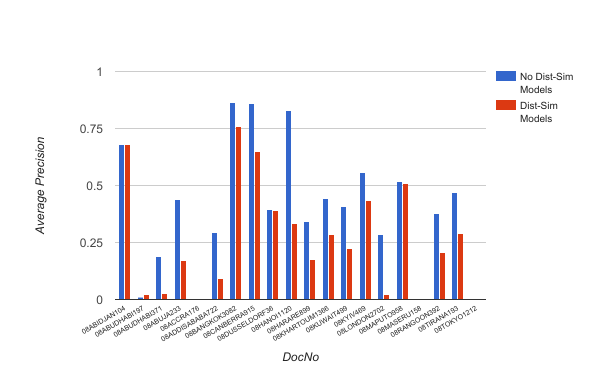
\includegraphics[scale=0.60]{images/query_by_query}
\caption{Comparison of Query Precision using Different NE Models}
\label{query_by_query}
\end{figure}
\subsection{Can we make the Tf-Idf Query Perform Better?}
\subsection{What makes a query good or bad?}
The queries formed from source documents \code{08ACCRA176} and \code{08MASERU158} score 0 precision in all four categories. This can be put down to the content of both of these documents. \code{08ACCRA176} describes a meeting of Ghanaian official following the raid of a brothel and \code{08MASERU158} describes a public transportation dispute. These stories are very local and so the number of relevant documents to find in the target collection will be vanishingly slim. \\
A single word can throw off the search results. ``Congress''. \\

\paragraph{Precision at 1}
\paragraph{Precision at 4}
At any given time, one can typically view 4 target documents in the search results page of the web application. It is interesting, then, to gather information on the precision of the top 4 documents returned when querying.

\paragraph{per-query scatterplot of source document length vs average precision of different query representations}

\subsection{Conclusion} 
Although the All Terms Query produced the highest MAP scores, it took upwards of 5x as long to run compared to the Named Entities query. At this point, we must weigh up the importance of relative result relevance against time concerns. Users are only willing to wait so long for results (Google and Microsoft suffer business impacts for 0.5s delays! \cite{performance}). The most highly performing queries consist of more terms and take longer to progress, although even this has diminishing returns.
As such, the most appropriate query to run automatically is that which consists of Named Entities.
\todo{Can we use both target indexes?}
Is it unreasonable to use both the distim and no-distim indexes depending upon the query being run? - It provides an improvement to the Tf-Idf named entities and subject queries.

\section{User Evaluation} \label{userevaluation}
\subsection{Think-Aloud}
Timothy Gollins, a key potential beneficiary of such a system participated in a small think-aloud study while examining the software in use. As former Head of Digital Preservation at The National Archives (UK), and current Head of Digital Archiving at the National Records of Scotland, Timothy has expert insight into the problem domain.
Some of the key points learned from this session are listed below:

\begin{itemize}
\item \textit{``Named Entity importance is nuanced and frequency (or Tf-Idf) of named entities does not necessarily produce the most important terms.''}
\par
This raises an important point regarding the limitations of automatic query generation.\textbf{There is of course the ability to run custom queries. But this could be improved somewhat}

\item \textit{``Further term highlighting or importance weighting is necessary to help produce the best results.''}
\par
This point highlight the fact that the queries generated right now are fairly general, and with some deep understanding of the way archivists review documents could help produce better results. Briefly mentioned was weighting the first and last paragraphs higher than the middle of the document, as these are likely to contain the most pertinent information.

\item \textit{``More advanced methods could be leveraged to improve yet further the capabilities of the software, like eye tracking or automatic querying upon highlighting''}
\par
Although beyond the scope of this project, this point identifies the potential expansion of this project. Eye-tracking could be used to automatically track what the user is interested in from the source document, forming the basis of new automatic queries. A simplified version of this could use text highlighting to accomplish the same results.

\item \textit{``UI considerations are equally as important as information retrieval considerations when it comes to improving the effectiveness of the software''}
\par
At this point in the project, the implementation of most of the IR functionality was complete. It now became important to consider how best to modify and improve the user interface to ensure the easiest experience possible. - DECORATION
\end{itemize}

\textbf{Talk about how this allowed iteration and improvement}

\section{Refining the System}
What did we do to make the system better:
Chose the best query.
Improved the stopwords file slightly.

What could we do to make the system better
Add yet more stopwords
Consider dates.

%%%%%%%%%%%%%%%%%%%%%%%%%%%%%%%%%%%%%%%%
\chapter{Conclusions} \label{conclusion}
\section{Fulfilled Requirements}
The Identifying Public Domain Knowledge project set out to create a system capable of improving the document review system necessary as digital records become more and more widespread.
The final product satisfies all of the Must Have requirements and addresses some of the Should and Could Have sections. 
\section{Possible Improvements}
Machine Learning. Eye Tracking. More Query formulations to analyse.

\section{Reflection}

%%%%%%%%%%%%%%%%
%              %
%  APPENDICES  %
%              %
%%%%%%%%%%%%%%%%
\begin{appendices}  r

\end{appendices}

%%%%%%%%%%%%%%%%%%%%
%   BIBLIOGRAPHY   %
%%%%%%%%%%%%%%%%%%%%

\bibliographystyle{plain}
\bibliography{bib}

\end{document}
